\documentclass{beamer}
\usepackage[utf8]{inputenc}
\usepackage[english,russian]{babel}
\usepackage{graphicx}
\usepackage{sidecap}

%beamer  theme's used to be here :)
\usetheme{mipt_beamer}

\title{Применение взаимодействующих нейронных сетей в криптографии}
\author{Ходаков Дмитрий.}
\date{March 14, 2014} %\today

\begin{document}
\frame{\titlepage}
\frame{\tableofcontents}

\section{Постановка задачи}

\subsection{Передача ключей}

\begin{frame}
\frametitle{Передача ключей}
\begin{itemize}
\item Безопасная замена алгоритма Диффи-Хеллмана
\item Основана на синхронизации двух нейросетей
\item Они называются древовидных машин четности (TPM, tree parity machines)
\end{itemize} 
\end{frame}

\subsection{Tree Parity Machines}

\begin{frame}
\frametitle{Tree Parity Machines}
\begin{itemize}
\item Многоуровневая нейронная сети прямого распространения
\item Входные нейроны принимают значения -1, +1
\item Веса между скрытыми нейронами принимают значения [-L, +L]
\item Значения скрытого нейрона ч= сигн w*x
\item Значения выходного нейрона т = ...
\end{itemize} 
\begin{center}
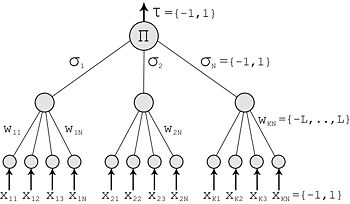
\includegraphics[width=5cm, height=5cm]{../../pics/tpm.jpg}
\end{center}
\end{frame}

\begin{frame}
\frametitle{Tree Parity Machines - алгоритм}
У каждого абонента (А или Б) есть своя TPM. 
Синхронизация:
\begin{itemize}

\item Задаём случайные значения весовых коэффициентов
\item Выполняем следующие шаги, пока не наступит синхронизация
\item Генерируем случайный входной вектор X
\item Вычисляем значения скрытых нейронов
\item Вычисляем значение выходного нейрона
\item Сравниваем выходы двух TPM:
\item Выходы разные: переход к п.2.1
\item Выходы одинаковые: применяем выбранное правило к весовым коэффициентам
\end{itemize} 

Для обновления весовых коэффициентов могут использоваться следующие правила:

Правило Хебба:
\(w_i^+=w_i+\sigma_ix_i\Theta(\sigma_i\tau)\Theta(\tau^A\tau^B)\)
\end{frame}

\section{Результаты}
\subsection{Зависимость скорости сходимости от eta}
\begin{frame}
\frametitle{Зависимость скорости сходимости от L}
Посмотрим, какова скорость схождения сети в зависимости от константы обучения.

\begin{center}
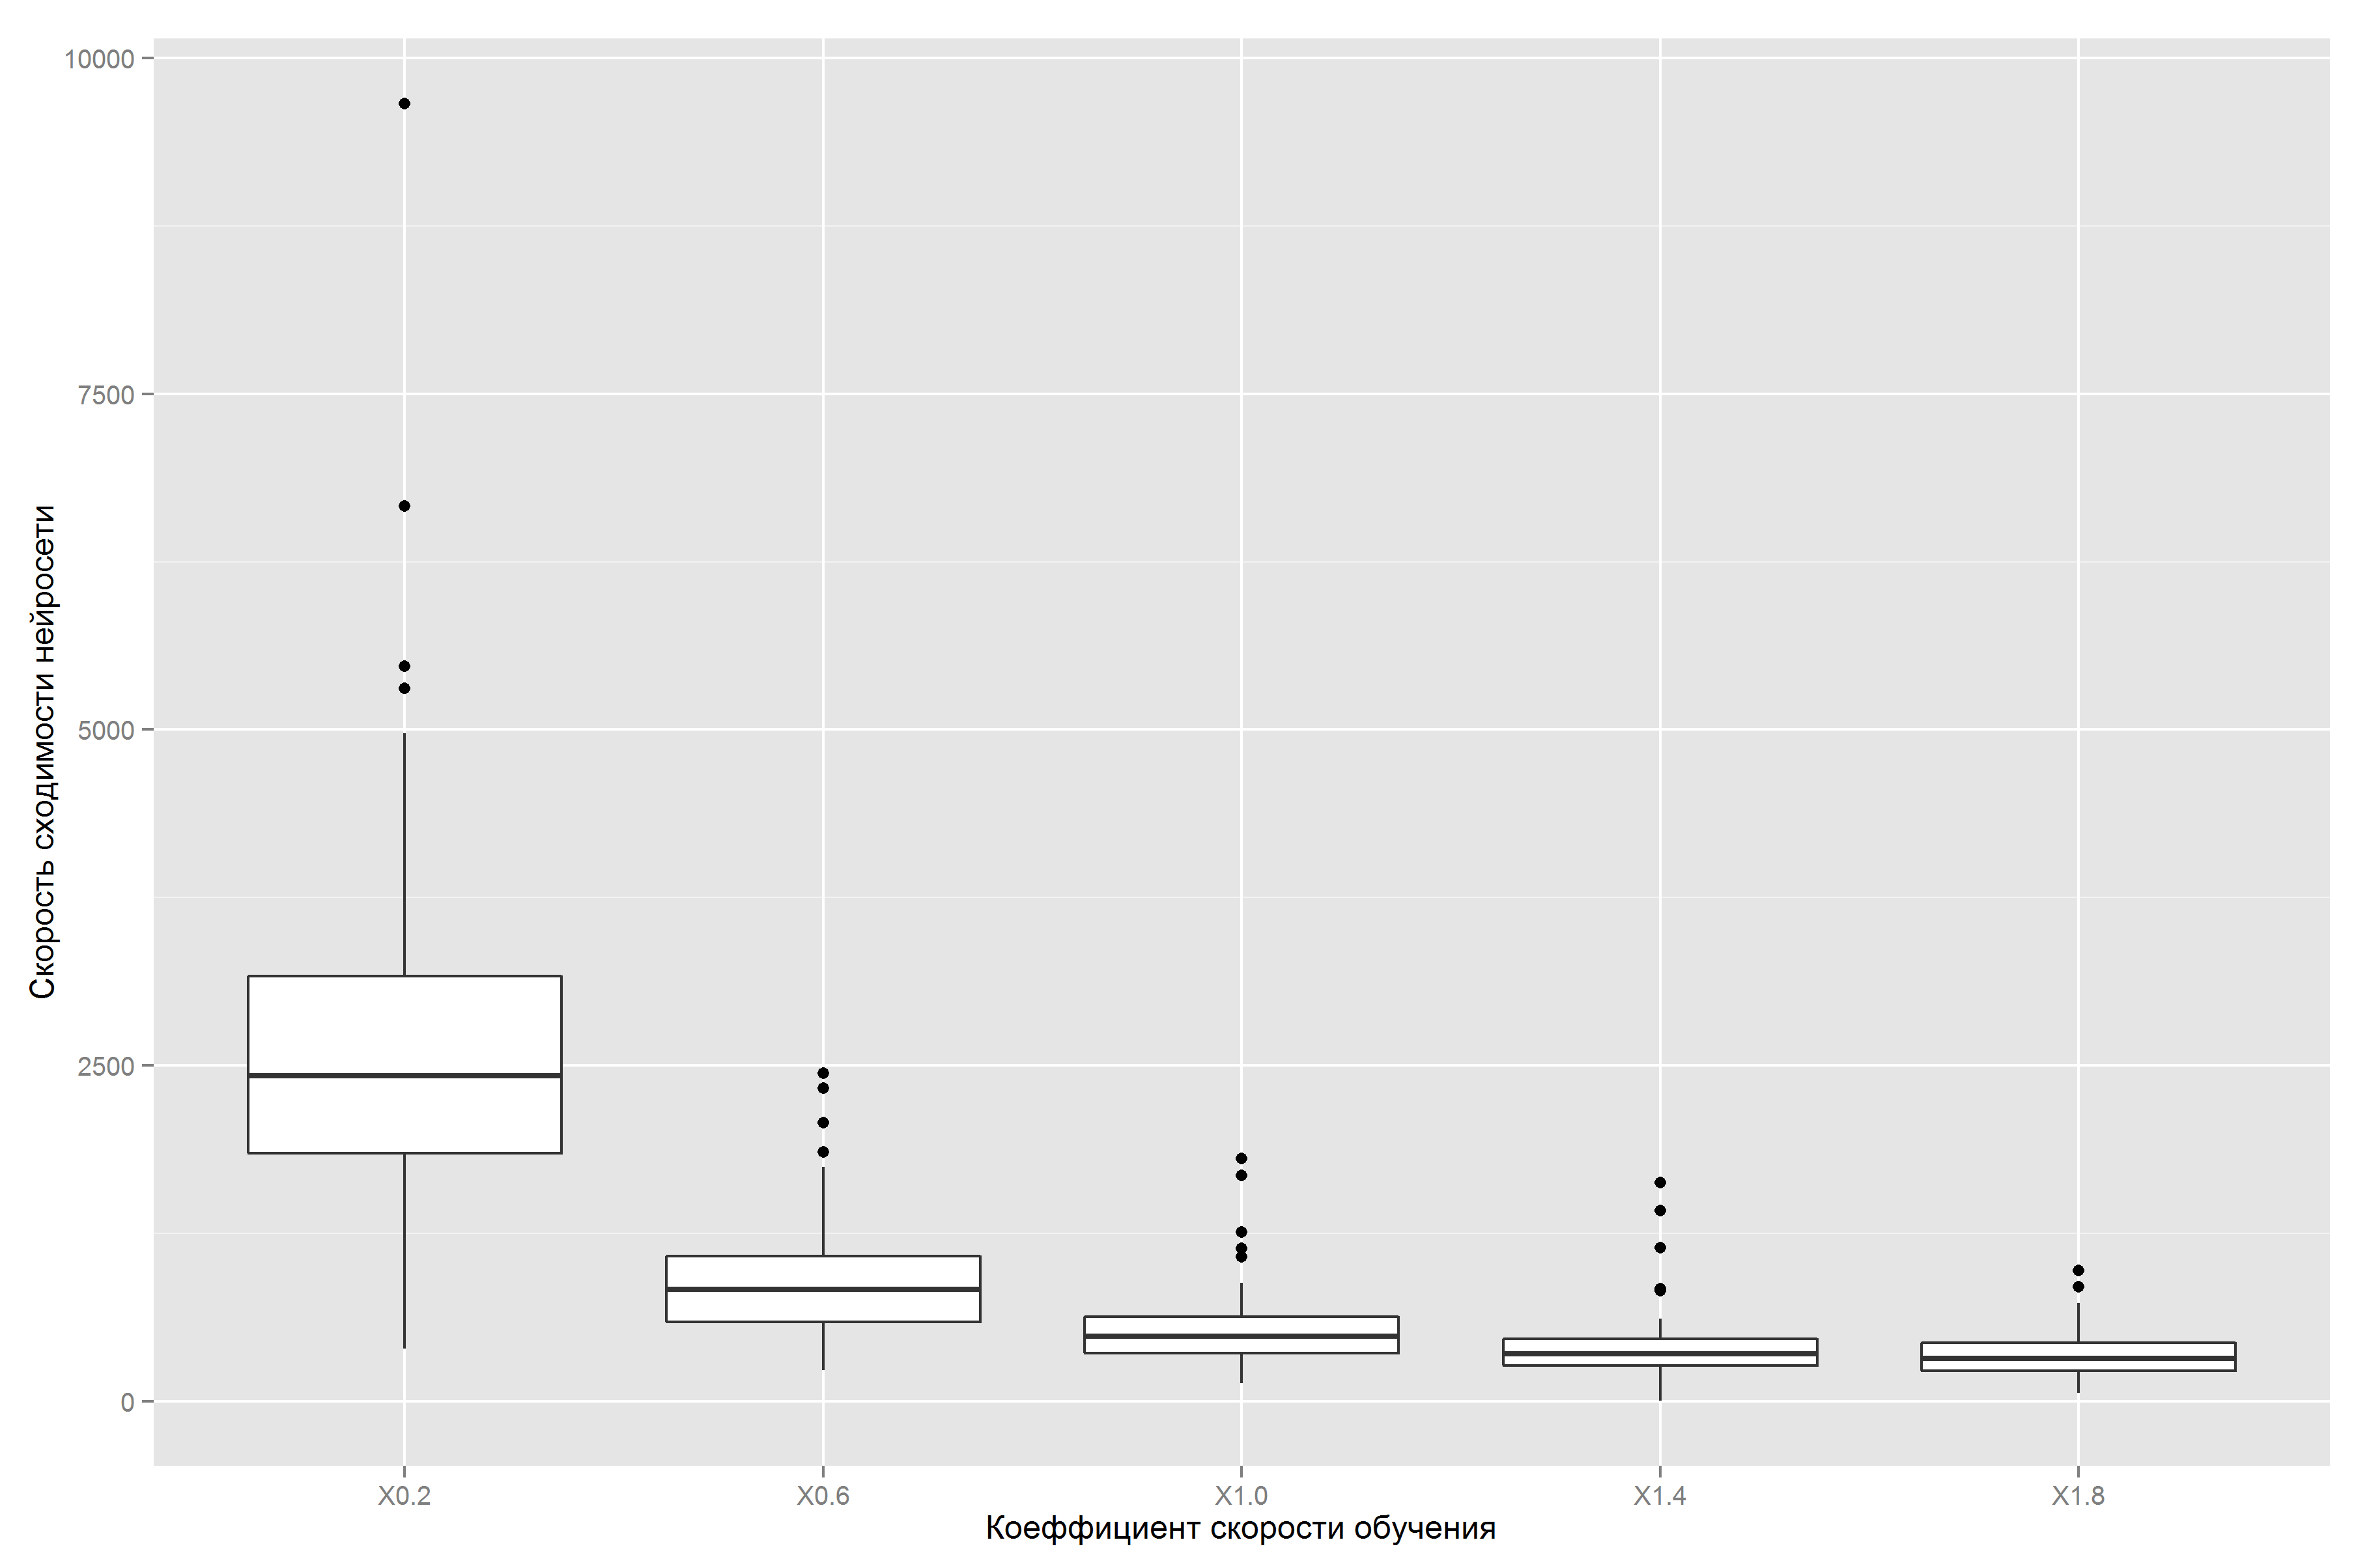
\includegraphics[width=5cm, height=5cm]{../../plots/eta_vs_speed.png}

\end{center}
\end{frame}

\subsection{Зависимость скорости сходимости от L}
\begin{frame}
\frametitle{Зависимость скорости сходимости от L}
Посмотрим, какова скорость схождения сети в зависимости от константы обучения.

\begin{center}
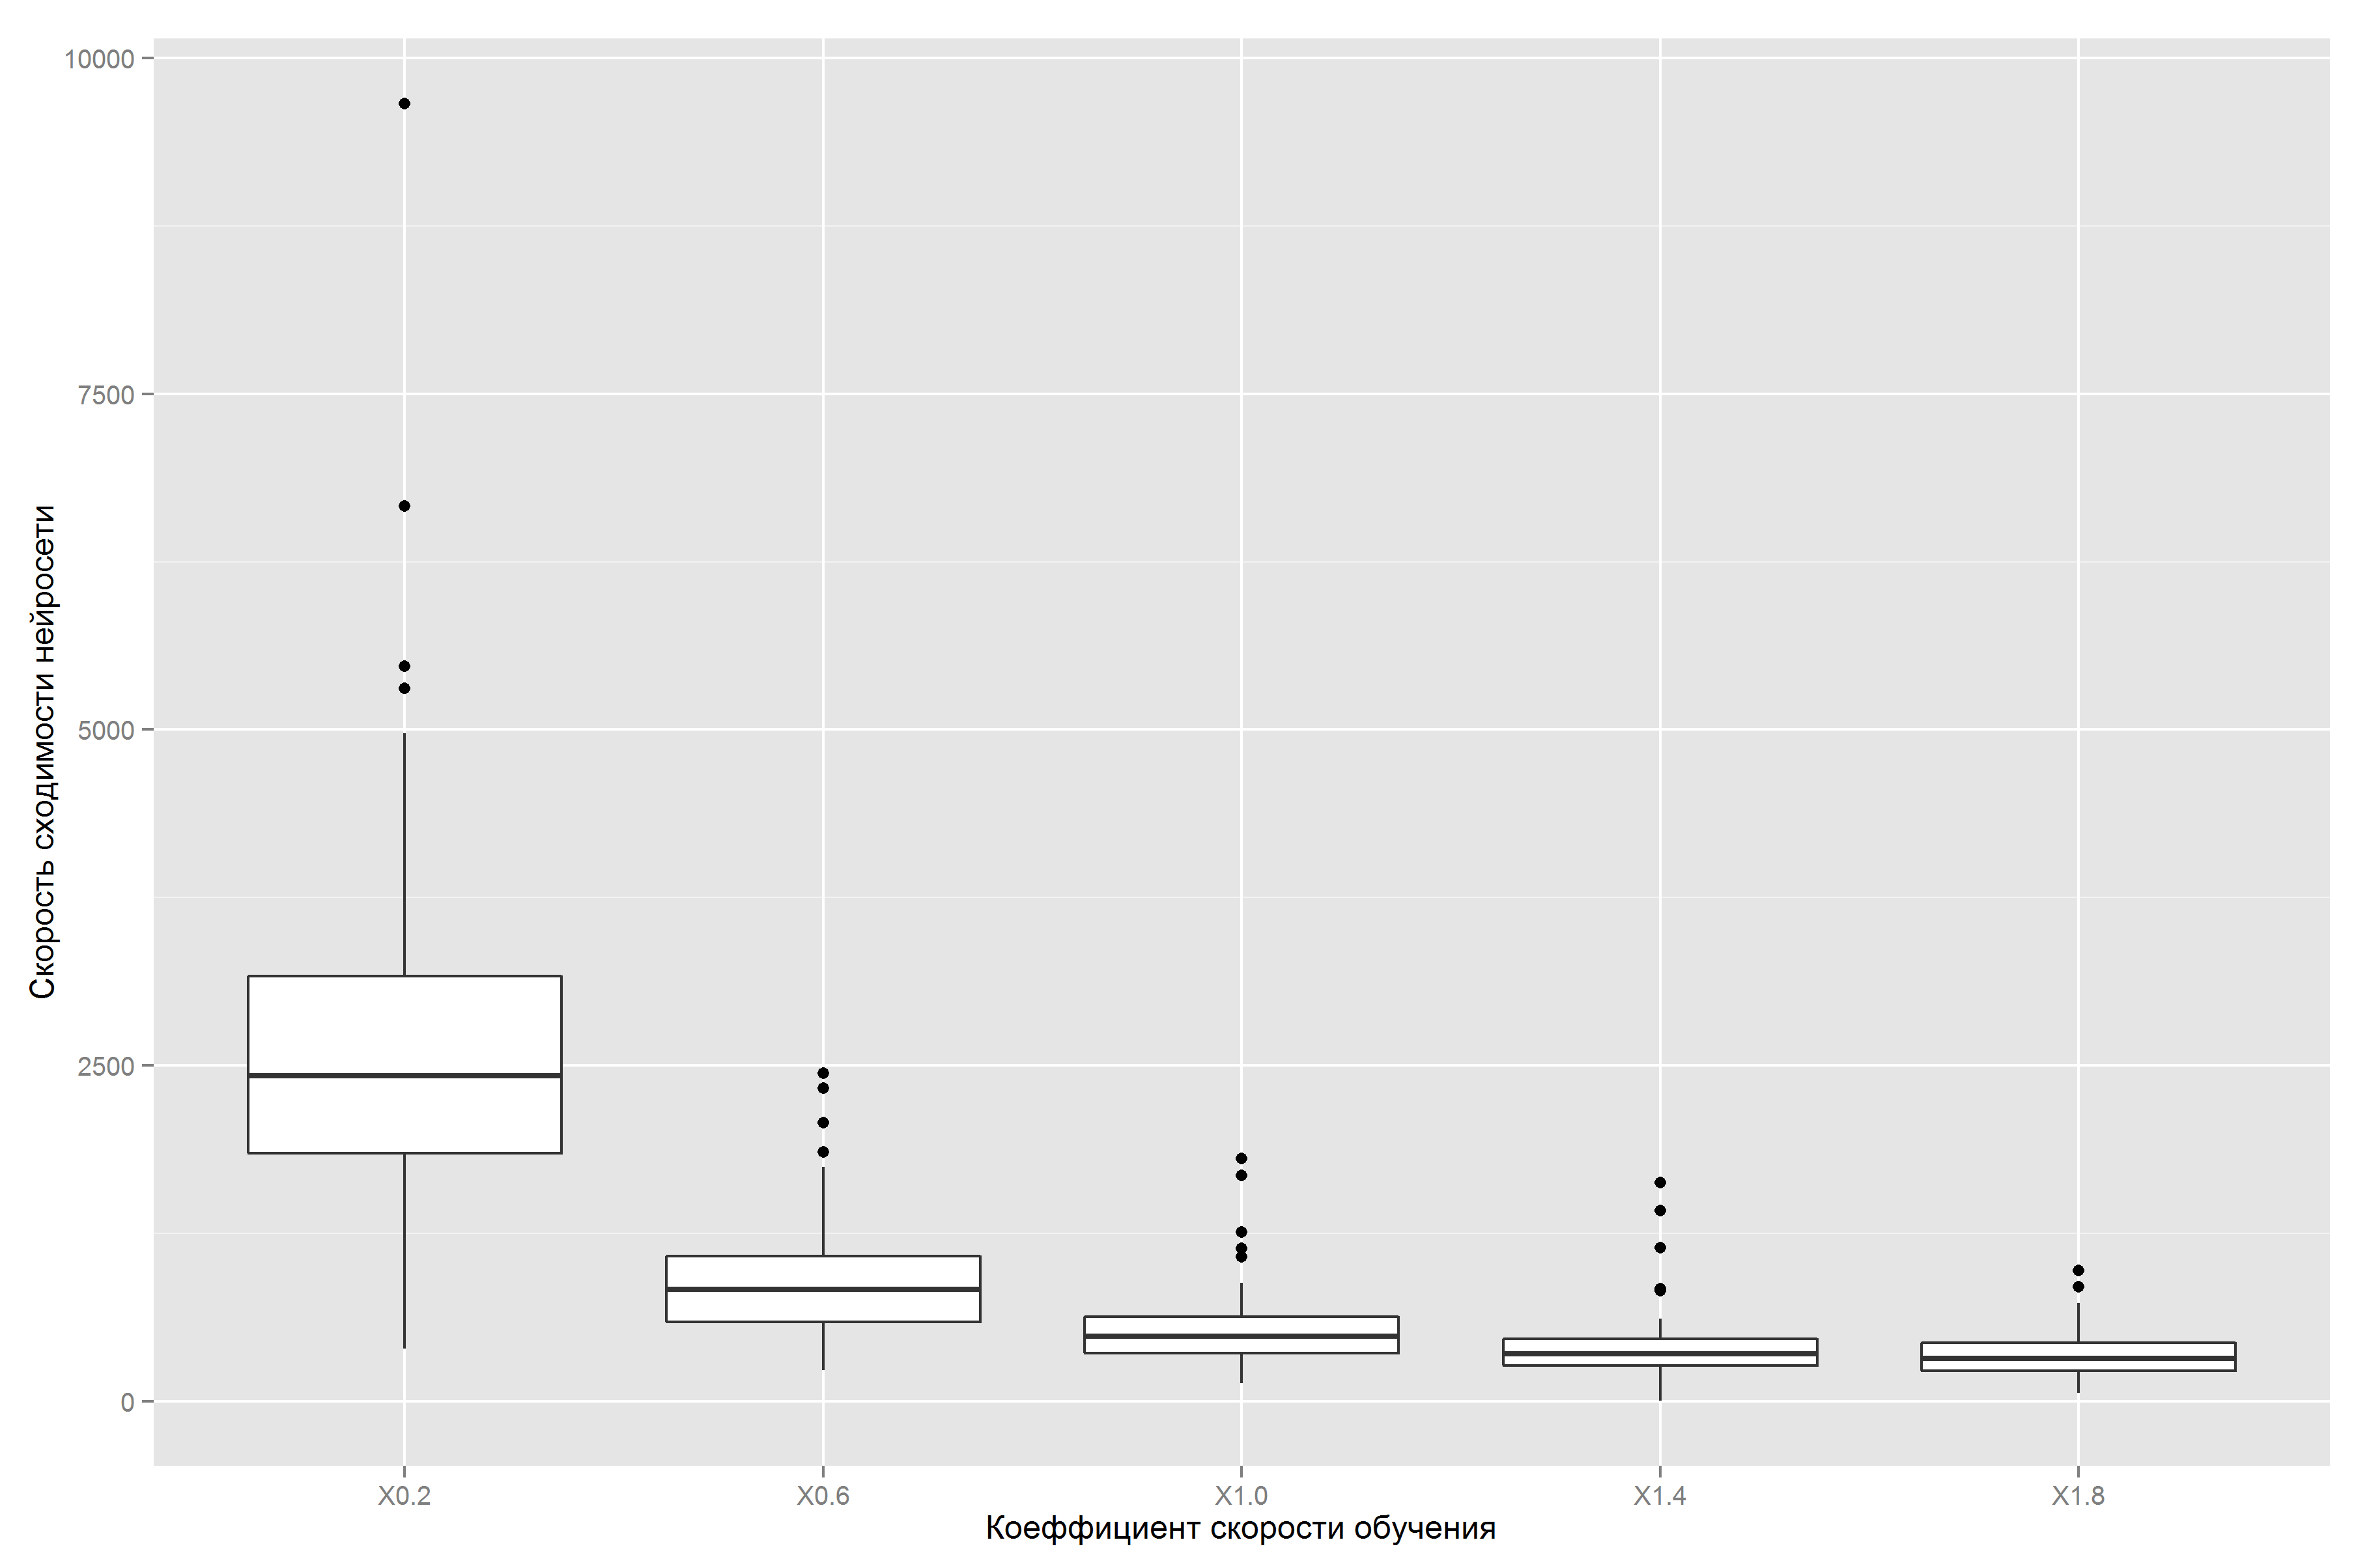
\includegraphics[width=5cm, height=5cm]{../../plots/eta_vs_speed.png}

\end{center}
\end{frame}

\subsection{Теоретическая формула для скорости обучения}
\begin{frame}
\frametitle{Теоретическая формула для скорости обучения}
Посмотрим, какова скорость схождения сети в зависимости от константы обучения.

\end{frame}

\subsection{Теоретическая формула оптимального времени синхронизации}
\begin{frame}
\frametitle{Теоретическая формула оптимального времени синхронизации}
Посмотрим, какова скорость схождения сети в зависимости от константы обучения.

\end{frame}
\end{document}

\subsection{Эффективность по ср с другими средствами криптографии}
\begin{frame}
\frametitle{Теоретическая формула оптимального времени синхронизации}
Посмотрим, какова скорость схождения сети в зависимости от константы обучения.
* насколько длина ключа влияет ln pn
\end{frame}
\end{document}